\chapter{Proposed algorithm}


The proposed algorithm was developed using lexical similarity algorithm combined with some of existing techniques, which are n-gram matching, lexical extensions. However, the way of computing passage scoring pays more attention to the specifications of meeting transcripts, which will be presented in detailed in the following sections.

Our system proceeds in three stages: (i) In the first stage, known as a pre-processing, the two questions and meeting transcripts are normalized and reorganized in order to enhance the performance of the algorithm; (ii) The second stage identifies a section of the meeting transcript which is most likely to contain the answer (i.e. evidence deciding the true and the false statement); and (iii) The third stage compares the two candidate statements with respect to the identified paragraph(s), and returns the true one. 


Figure \ref{SystemOverview} gives an overview of the 3 stages.

\begin{figure}[htbp]
\centering
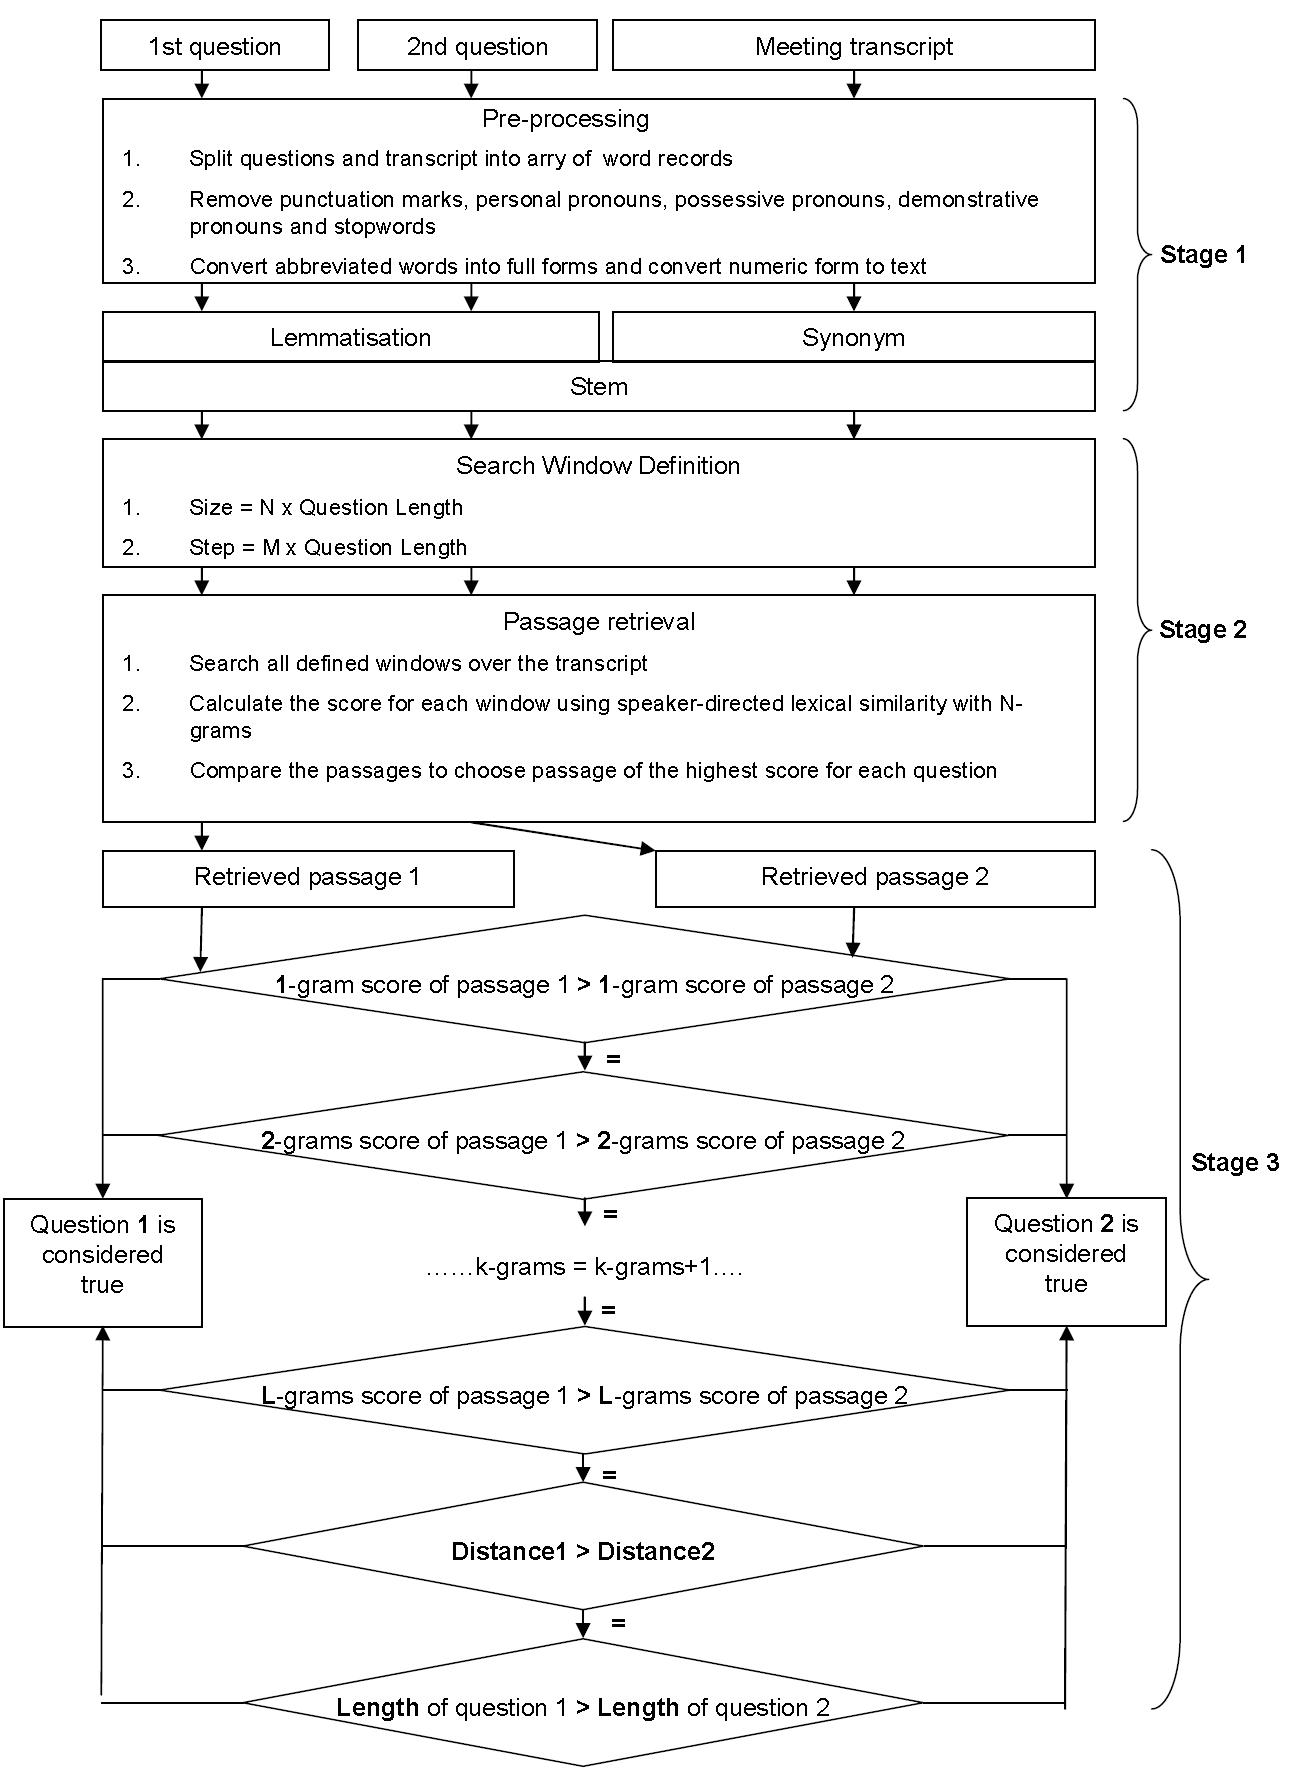
\includegraphics[scale = 0.6]{Stages_of_system.jpg}
\caption{Overview of the system}\label{SystemOverview}
\end{figure}


%Figure \ref{SystemOverview}



\section{Pre-processing}
There are two main tasks for this section. First, questions and transcript are transformed into the same form of written text so that they can be compared word by word later. Secondly, in order to enhance the probability of matching between two words, each word is extended by lemma, stem and synonyms.

The first processing is done by five operations as follows:

\begin{enumerate}
\item {Removing characters as punctuation marks: comma, dot, quotation mark, semicolon or exclamation, \ldots because these characters do not have any effects on the proposed algorithm based on lexical similarity. } 

\item {Removing stopwords such as "the", "to" or "for" that generally add little or no information regarding the subject matter of text \cite{mckechnie2001cap}.  This helps to reduce cost of computing as well as to take precaution that they muddle the signal from the more content words \cite{hirschman1999drr}}

\item {For the reason that the questions are indirect-speech statements meanwhile the the meeting transcript is a direct-speech report, words that may be changed for a transformation from direct speech to indirect speech should be avoided from counting matched words between a question and a passage because this leads to lexical mismatches. They are personal pronouns (I, me, myself, you, \ldots), possessive pronouns (my, your, \ldots), demonstrative pronouns (this, that, \ldots).}



\item {Converting numeric forms to text forms: 34 \ensuremath{\rightarrow} thirty four, 2nd \ensuremath{\rightarrow} second, etc. \ldots so that they are written in the same way, this prevents an unnoticed matching while the algorithm executes. }

\item {Converting abbreviated words into full forms: We've \ensuremath{\rightarrow} We have, I'll \ensuremath{\rightarrow} I will, etc. \ldots. This operation helps the system treat the text in the same way.}
\end{enumerate}

All words are transformed into lower-case forms so that nouns, pronouns and verbs have the same level of importance. That means parts-of-speech will not be used to assign scores to words in the Passage Retrieval stage.

The proposed algorithm uses lexical similarity to find a relevant passage that contains answer information (Section 4.2). Thus, a lexical extension should be added so that the system has more than one matching possibility between two words. Take the words \textit{production} and \textit{product} as examples, they match each other because they have the same stem as \textit{produc}.

Three lexical extensions are added to each word, including lemma, stem and synonym. 
\begin{itemize}
\item {Lemma is the canonical form of the word.}
\item {Stem is used to remove inflectional affixes.}
\item {Synonyms have same meaning with the original word.}
\end{itemize}

However, it is not suitable to apply all these extensions to both questions and the transcript. For instance, if both question words and answer word are extended by a set of synonyms, it can create a so called "redundant information". In addition, it may make the result of the algorithm inaccurate if they are considered similar because of similarity of an intermediate synonym. For example: \textit{meeting} and \textit{challenge} have one synonym \textit{contest} in common, but they do not have the same meaning. For that reason, a question word is extended by adding its lemma, meanwhile the transcript words are extended by adding a set of synonyms. Meanwhile, stem is applied as the last operation on each word. This may increase the signal from words. For instance with such a question word as the verb \textit{modified} and such a transcript word as the noun \textit{modification}, there are not any matching between these words, even after adding a lemma and a synonym.  In detail, \textit{modified} becomes \textit{modify} by a lemmatisation and \textit{modification} has five synonyms \textit{alteration, adjustment, qualifying, limiting, change} (returned by WordNet \cite{pasca2001irw}). But after stemming by Snowball \cite{porter2001ss}, these two words will have a same form as \textit{modifi}, so they are matched.

In practice, for each word, the program runs a Stemming API of Porter, called Snowball \cite{porter2001ss} to obtain a stem and WordNet API \cite{pasca2001irw} to obtain a lemma and a set of synonyms.

A set of synonyms is reduced to be more coherent with the original word by using parts of speech (PoS) tool named QTAG API \cite{manson1997qpp}, which aims at removing synonyms that do not have the same PoS as the original word.

Therefore, each word will be treated from now on as a record of many fields. For a question word, it has three fields: original word, lemma of the word and stem of the lemma. They are described in the Table \ref{Word splitting and lexical extensions for questions}. The format of input transcript as described in the Tables \ref{transcript_IB4010} and \ref{transcript_IS1008c} helps the program identify the speaker of any word in the transcript. Hence, a record of a transcript word has five fields: original word, stem of word, name of speaker name who spoke this word, set of synonyms and part of speech. They are described in the Table \ref{word_splitting_transcript}. The name of speakers is also stemmed in order to compare with a question word which may be a speaker name. This field is very important to assess a statement with respect to a specific speaker.

The fields \textit{synonyms} and \textit{lemma} are structured as a set of words because they may have more than one element. For example, lemma of "better" has two words \textit{good} and \textit{well}, synonyms of \textit{better} are \textit{break}, \textit{improve}, \textit{amend}, \textit{ameliorate} and \textit{meliorate}.


For instance, for the pair of such questions as \textit{Mirek had not received the agenda for the meeting} and \textit{Andrei had not received the agenda for the meeting}, after removing stop-words, they remain \textit{Mirek had not received agenda meeting} and \textit{Andrei had not received agenda meeting}. Their lexical extensions are presented as following table:
\begin{table}[htbp]
\scriptsize
\caption{Word splitting and lexical extensions for questions}
\begin{tabular}{|c|l|l|l|l|c|l|l|l|}
\hline
\multicolumn{ 4}{|c|}{\textbf{Question 1}} &  & \multicolumn{ 4}{c|}{\textbf{Question 2}} \\ \hline
\textbf{Position} & \multicolumn{1}{c|}{\textbf{Word}} & \multicolumn{1}{c|}{\textbf{Lemma}} & \multicolumn{1}{c|}{\textbf{Stem}} &  & \textbf{Position} & \multicolumn{1}{c|}{\textbf{Word}} & \multicolumn{1}{c|}{\textbf{Lemma}} & \multicolumn{1}{c|}{\textbf{Stem}} \\ \hline
1 & Mirek & Mirek & Mirek &  & 1 & Andrei & Andrei & Andrei \\ \hline
2 & had & have & have &  & 2 & had & have & have \\ \hline
3 & not & not & not &  & 3 & not & not & not \\ \hline
4 & received & receive & receiv &  & 4 & received & receive & receiv \\ \hline
5 & agenda & agenda & agenda &  & 5 & agenda & agenda & agenda \\ \hline
6 & meeting & meet & meet &  & 6 & meeting & meet & meet \\ \hline
\end{tabular}
\label{Word splitting and lexical extensions for questions}
\end{table}

\normalsize



One example for a snippet of transcript as below:
\scriptsize
\begin{verbatim}
.....
 Andrei Hi everyone. 
 Denis  So I don't know if you all received the the a- agenda for this meeting.
 Denis 	Do you - no?
 Mirek 	No, I haven't.
....
\end{verbatim}
\normalsize

After the processing, it remains:
\scriptsize
\begin{verbatim}
.....
denis   9 not 10 know 11 if 12 you 13 all 14 received 18 agenda 21 meeting
denis   24 no 
mirek   25 No 27 have 28 not
....
\end{verbatim}
\normalsize

and it is transformed into the following table:

\begin{center}
\begin{threeparttable}
\scriptsize
\caption{Word splitting and lexical extensions for transcript}
\label{word_splitting_transcript}
\begin{tabular}{|c|l|l|c|l|l|}
%\hline \multicolumn{6}{|c|}{Word splitting} \\
\hline  \bf{Position} & \bf{Word} & \bf{Stem} & \bf{Speaker} & \bf{Synonyms (stemmed)} &\bf{PoS} \\
\hline \ldots & \ldots & & & &\\
\hline 9 & not & not & deni & non & XNOT\\
\hline 10 & know & know & deni & cogniz experi live acknowledg recogn \ldots & VB\\
\hline 11 & if & if & deni & & CS\\
\hline 13 & all & all & deni & entir complet total altogeth whole  \ldots & PDT\\
\hline 14 & received & receiv & deni & have get find obtain \ldots &VBD\\
\hline 18 & agenda & agenda & deni & docket schedul agendum \ldots & NN\\
\hline 21 & meeting & meet & deni & fill match ensembl contact \ldots & NN\\
\hline 24 & no & no & deni & nobelium & DT\\
\hline 25 & no & no & mirek & nobelium & DT\\
\hline 27 & have &have &mirek &  receiv get own possess \ldots &HV\\
\hline 28 & not &not &mirek & non&XNOT\\
\hline \ldots & \ldots & & & &\\
\hline 
\end{tabular}
\end{threeparttable}
\end{center}


\normalsize

All of the steps above are processed in a procedure separated from execution of the main algorithm, which consists of passage retrieval and true-false answer. The questions and the transcript pre-processed from this stage are stored on hard disk so that the programme can load them into RAM before running the main algorithm. This saves us much time to experiment on different configurations of the algorithm that requires the repeatition of execution with the same input data.

\section{Passage retrieval} 

% definition of a passage must be mentioned in the state-of-the-art

The main goal of this stage is to narrow the space of searched answer by locating a passage which is considered the most likely to contain all the information about the answer, like evidence that helps to discriminate the true statement from the false statement in a pair. It also gives a numeric score indicating the similarity level between a found passage and the question so that two complementary statements in a pair may be compared in the subsequent stage.

In order to find the relevant passage, the system has to compare all possible passages in the transcript. Information being compared is passage scoring, which is a numeric value used to measure the level of similarity between a passage and a question. This task is done by moving a search window from one place to another over the entire transcript. If we assume that the transcript is a cloth stretched to be ironed, then the search window is the iron. In the same way of using an iron, the search window passes over all possible passages that have the same size as the search window in the transcript. All of the retrieved passages by this way are compared in order to provide the passages of highest score \cite{lequocanh}. 

As listed in the Chapter 2, there are many ways to calculate the score of a passage with respect to the question. According to the experimental results of Stefanie \cite{tellex2003qep} with different algorithms of passage retrieval, the performance of the algorithms is different from each other depending on input data. That means each method is suitable for only certain cases. Moreover, existing passage retrieval algorithms use input retrieved by a document retrieval that returns unknown-typed documents such as a forum website, a commercial website or an online newspaper, etc. Additionally, these approaches have to analyze the type of questions such as \textit{How} or \textit{When} before the stage of passage retrieval  \cite{TREC8, TREC2001, hirschman2002nlq, tellex2003qep}. This effects the final results of the passage retrieval algorithm because each step accumulates a certain error. In our case, the type of document and the type of questions are defined before, as described in Chapter 3. That is why we do not apply any existing complex algorithms, but rather develop our own algorithm based on the basic one presented by Light et al. \cite{light2002aec}. The method of Light is the simplest method to calculate a passage scoring, which is the number of matched words between the passage and the question. Based on this method, we added some certain extensions to the original algorithm, including n-gram matching, lemmatisation, stem, synonyms and various scores assigned to matched word. Lexical extensions such as lemmatisation, stem and synonyms have been presented in the previous stage while the application of n-gram matching and different scores are to be explained specifically in following sections.

As described by Light et al, the score of a passage is based on the number of matched words. However, there are three score levels assigned to matched words. As illustrated in the table \ref{word_splitting_transcript}, each word from the transcript corresponds to one speaker's name. Therefore, if a matched word is spoken by a speaker whose name is addressed in the question, the score assigned to this word must be higher than other matched words. 

In our experiment system, as presented in the pseudo code \ref{alg: Passage Score}, different values of score are assigned to a matched word as follows: 
\begin{enumerate}
\item {If a word from the question matches the name of the speaker in the passage, then it receives the highest score (e.g., 4.0)}
\item {If a word from the question matches a word from the passage (lemmas), and this word is spoken by a speaker mentioned in the question, then it receives the second highest score (e.g.,2.5)}
\item{Otherwise, if a word from the question matches a word from the passage (lemmas) then it receives the "normal score" (e.g.,1.0)}
\item{If a word (lemma) from the question matches one of the synonyms of a word from the passage, then it receives a "low" score (e.g.,0.5)}
\end{enumerate}

The numeric values listed above are set by the author based on the intuition about the importance of each matching, and might not be optimal for this task. No automatic optimization (statistical learning) could have been attempted because the amount of data was insufficient.


As mentioned above, a search window is used to seek and calculate all possible passages on the transcript. The size of the search window is defined as a multiple of the question length. Meanwhile, the distance between two consecutive windows is known as window step and also defined as a multiple of question length. For instance, window size = 5 x question size and window step = 2 x question size. Thus, parameters of search window are dynamic depending on the input question length. This method seems suitable to retrieve relevant passages using the lexical similarity algorithm because when the length of the question increases, the information that the question demands is larger. As a result, it is necessary to enlarge the size of search window.

The passage retrieval algorithm returns a list of passages at the same highest score. Nevertheless, we would like only one passage for the next stage of the algorithm because it is likely that only one relevant passage corresponds to each BET question. In order to choose the most relevant passage, 2-gram score, 3-gram score and so on until n-gram score are compared to reduce the number of passages in the returned list, in which n is the number of question words. A k-gram score is calculated as follows: Instead of working with matched words between question and answer, the program will work with matched substrings of k words between them. If two passages have same 1-gram score, their 2-gram score are compared with each other to return higher-score passages. If they have the same 2-gram score, their 3-gram score are compared with each other. This continues in the same way until one passage has a higher score than others or all n-gram scores are compared with each other, in which n is the number of words in the question. If they still have same n-gram score, the first passage is returned. In fact, n-gram matching is the simpler variant of the dependency relation approach among matched words that the matching of words in order is better.



The implementation of passage scoring calculation is described by pseudo code \ref{alg: Passage Score} with comments in detail. The following is a list of the most impotant features of this implementation:

- A passage is defined as a class that has 5 properties: 1) Passage score, which indicates the similarity between this passage and the current question. The passage score is computed as the sum of the scores for each matched word; 2) Position of the passage in the transcript; 3) Size of passage; 4) Set of positions of matched words in the transcript; and 5) Distance among matched words (density). This distance is calculated as the sum of absolute distance between any two matched words. This task is done at the end of the passage retrieval to prepare for the True-False Answer stage.


- The order of priority is to "name matching", then "stem matching" and lastly "synonyms matching" in order to compute the highest score for the current passage.

- The frequency of one matched word is not used to increase the score. However, in the case of "multiple matching", if one word is repeated more than one time in both the question and the passage, the number of matched words will be counted as the minimum number of appearance of this word in both the question and the passage. 



\newpage


% Chia lam 2 cot, cot ben phai dung de viet comments
\begin{algorithm}                      % enter the algorithm environment
\caption{Passage Retrieval}          % give the algorithm a caption
\label{algo: Passage Retrieval}                           % and a label for \ref{} commands later in the document
\begin{algorithmic}       [1]             % enter the algorithmic environment
\scriptsize
\REQUIRE Question \COMMENT {Array of word records as described in the table \ref{Word splitting and lexical extensions for questions}}
\REQUIRE Transcript \COMMENT{Array of word records as described in the table \ref{word_splitting_transcript} }
\REQUIRE WindowSize \COMMENT {Size of search window (in word unit)}
\REQUIRE WindowStep \COMMENT{Distance between two consecutive windows (word unit)}

\STATE $Passage \gets Empty$ \COMMENT{Initiate a new passage as current passage(the passage class is defined above)}
\STATE $BestPassage \gets Empty$ \COMMENT{Initiate a new passage as the best retrieved passage at one moment}

\STATE $Position \gets 0$ \COMMENT{Initialized position of the search window}
\WHILE[Search for all passages to choose the best passage]{$Position \ensuremath{<} Transcript.length-WindowSize$} 
	\STATE $Passage.position \gets Position$ \COMMENT{Position of current passage}
	\STATE $Passage.size \gets WindowSize$   \COMMENT{Size of current passage}
	\STATE $Passage.WordList \gets Transcrip[Postion \div Position+WindowSize]$ \COMMENT{List of word records is extracted from the transcript[Position,Position+1,..,Position+Size of window]}
	\STATE $Ngrams \gets 1$ \COMMENT{Firstly, passage score is calculated using unigram matching}	
	\STATE $Passage.MatchedList \gets getMatchedList(Passage,Question,Ngrams)$ \COMMENT{that is from the procedure \ref{alg: Passage Score} }
	\STATE $Passage.score \gets getPassageScore(Passage,Question,Ngrams)$ \COMMENT{that is from the algorithm \ref{alg: Passage Score} }
	
	\IF[The current passage is better]{$BestPassage.score \ensuremath{<} Passage.score$} 
		\STATE $BestPassage \gets Passage$ \COMMENT{remember it as the best passage}
	\ELSIF[If they have the same score]{$BestPassage.score \equiv Passage.score$} 
		\WHILE[Recalculate their score using bigrams, trigrams,.. until their score is different from each other or Ngrams is over the length of question ]{$BestPassage.score \equiv Passage.score \wedge Ngrams \leqslant Question.length $}
			\STATE $Ngram \gets Ngrams+1$ \COMMENT{Increase Ngrams by 1}
			\STATE $BestPassage.score \gets getPassageScore(BestPassage,Question,Ngrams)$ \COMMENT{Recalculation with new Ngrams}
			
		\ENDWHILE
		\IF[Finally, if current passage have better score, remember the current passage as the best passage until now]{$BestPassage.score \ensuremath{<} Passage.score$} 
			\STATE $BestPassage \gets Passage$
		\ENDIF
	\ENDIF
	

	
	\STATE $Position \gets Position+WindowStep$ \COMMENT{Move the search window forward}
	
\ENDWHILE


%Distance
\STATE $Passage.distance \gets 0$
\FOR{$i=0$ to $Passage.WordList.Length-1$}
	\FOR{$j=i+1$ to $Passage.WordList.Length$}
		\STATE $Passage.distance  \gets Passage.distance + abs(Passage.MatchedList[i]-Passage.MatchedList[j])$		
	\ENDFOR
\ENDFOR
\RETURN BestPassage
\end{algorithmic}
\end{algorithm}


\normalsize






%\algsetup{indent=2cm}

\begin{algorithm}                      % enter the algorithm environment
\caption{Passage Score Calculation}          % give the algorithm a caption
\label{alg: Passage Score}                           % and a label for \ref{} commands later in the document
\begin{algorithmic} [1]                   % enter the algorithmic environment
\scriptsize
%\tiny \scriptsize \footnotesize \small \normalsize 
%\large \Large \LARGE \huge \Huge

\REQUIRE $Question[] \neq null$ \COMMENT{Array of word records as described in the table \ref{Word splitting and lexical extensions for questions} }

\REQUIRE $Passage.WordList[] \neq null$  \COMMENT{Array of passage word records as described in the table \ref{word_splitting_transcript}}

\REQUIRE $Ngrams \geqslant 1$   \COMMENT{1 for unigram; 2 for bigram; 3 for trigram}

\STATE $Score \gets 0$ \COMMENT{Initialization value for passage score}.
\STATE $Speaker \gets Null$ \COMMENT{Name of a speaker that is mentioned in the question}
\STATE $PositionsSet \gets Null$ \COMMENT{Set of matched word positions}
\STATE $AvailQues[] \gets True$ \COMMENT{Available status of each question word to match with passage words}
\STATE $AvailPas[] \gets True$ \COMMENT{Available status of each passage word to match with question words}


\STATE \COMMENT{Firstly, search for a speaker name that is containned in both question and passage}
\FOR{$i=0$ to $Question.length$}
	\STATE $Matching \gets False$
	\STATE $j \gets 0 $ 
	\WHILE{$!Matching \wedge j\leqslant Passage.WordList.length$}
		\IF[If one exists]{$Question[i].Stem \equiv Passage.WordList[j].Speaker$}
			\STATE $Score \gets Score + 4.0$ \COMMENT{Then passage score increases 4.0 points }
			\STATE $Speaker \gets Question[i].Stem$ \COMMENT{Remember this name for step later}			
			\STATE $AvailQues[i] \gets False$
			\STATE $Matching \gets True$
		\ENDIF		
		\STATE $j\gets j+1$ 
	\ENDWHILE
\ENDFOR

\STATE\COMMENT{Checking for a N-grams matching}
\FOR{$i=0$ to $Question.length$}
	\STATE $Matching \gets False$
	\STATE $j \gets 0$
	\WHILE{$!Matching \wedge j\leqslant Passage.WordList.length \wedge AvailQues[i] \wedge AvailPas[j] $}
		\STATE $Matching \gets True$
		\FOR {$k=0$ to $Ngrams$}
			\IF{$Passage[j+k].stem \nsubseteq Question[i+k].lemma$}
				\STATE $Matching \gets False$
			\ENDIF
		\ENDFOR
		
	\IF[If one exists]{$Matching$}
		\IF[Speaker of matching words is mentioned in the question]{$Speaker \equiv Passage.WordList[j].Speaker$}
		\STATE $Score \gets Score + 2.5$ \COMMENT{Then the score increases 2.5 points}
		\ELSE 
		\STATE $Score \gets Score + 1.0$ \COMMENT{Other cases, the score increases 1.0 point}
		\ENDIF
		\STATE $AvailQues[i] \gets False$ \COMMENT{These words will be disable from next matching process} 
		\STATE $AvailPas[j] \gets False $ 
				
		\STATE $PositionsSet \gets PositionsSet \cup j$ \COMMENT{Save position of matching to list}
	\ENDIF

		
	\STATE $j \gets j+1$
	\ENDWHILE
\ENDFOR

\STATE\COMMENT{Checking for a synonym matching}
\FOR{$i=0$ to $Question.length$}
	\FOR{$j=0$ to $Passage.WordList.length$}
		\IF{$Question[i] \subseteq Passage.WordList[j].Sysnonyms \wedge AvailQues[i] \wedge AvailPas[j]$}
			\STATE $Score \gets Score + 0.5$
			\STATE $PositionsSet \gets PositionsSet \cup j$ \COMMENT{Save position of matching to list}
		\ENDIF
	\ENDFOR
\ENDFOR

\RETURN Score, List
\end{algorithmic}
\end{algorithm}

\newpage
\normalsize




\newpage

\section{True-False Answer}

Based on two retrieved passages corresponding to two input statements from the previous stage, the purpose of this stage is to identify the true statement in a pair. 

At the first sight, this system seems simpler than other question answering systems, which must analyze the type of question, such as \textit{Who} or \textit{How} before extracting answer words in retrieved passages as mentioned in the Chapter 2. In our case, two questions in a pair are formed as statements and the answer is simply \textit{true} or \textit{false} one bit for each question. However, because two questions are very close with each other, that means that in most cases they are different from each other by only one or two words. Thus, it is not easy to distinguish one question from another, even when the retrieved passage corresponding to the true question is correct (the retrieved passage corresponding to the false question is always false because information of this statement does not exist in the transcript). The only hopefulness is that the passage corresponding to the false statement can help the system tell that the statement is false due to their number of matched words is less.

For passages retrieved from the previous stage, we have two cases: a passage corresponding to the true question is evaluated as incorrect or correct. In the first case, when both retrieved passages are incorrect, thus we cannot identify the true statement by any reasonable algorithm. This is because that the database, which are the passages, used to give the answer is not correct. In the second case, we also have two possibilities: (i) two passages are identified; and (ii) two passages are different from each other. For the second possibility, there is not relation between the first question and the second question. They are totally different. Their retrieved corresponding passages are therefore two different ones. As a result, the only way to answer which question is correct is to measure independently the correctness of each question based on their passage. Then, the question whose accuracy is higher is considered to be true. At this time, the question of how to measure them has to be answered? If we use passage score to evaluate them, there is not any reason that the number of matched words of the false question would be less than those of the true question. So this step needs a deeper analysis on semantic text to answer the question persuasively. We have not yet found an effective method to assess which question is "more" correct.

The proposed algorithm is applied rather in the case that both the two passages have the same position in the transcript. The possibility of this is high because the similarity of two statements in a pair as mentioned in Chapter 3. That means the same passage retrieved for both the true and the false candidates as well as the passage corresponding to the true question are correct. In this case, it is more probable that passage score of the false statement is less than this of the true statement. It is also the main idea of the proposed algorithm for this step. Despite the simplicity of this algorithm, experimental results are much better than results by chance (see section 6.2).

In detail, all scores for 1-gram matching, 2-gram matching, ..., n-gram matching of two passages are used to assess two questions. If two passages have the same 1-gram score, their 2-gram score will be compared, continuing in the same way until one passage have higher score or all n-gram scores were compared. In this case, n is number of words from the smaller question. In fact, using n-gram matching is the simplest version of using dependency relations between neighbor words. The way of calculating n-gram matching has been presented in the previous section Passage Retrieval. In the case they still have the same score, the number of words from two passages are then compared with each other. To explain, one question will be considered to be true if the number of matched words over the total number of question words is smaller.

Pseudo code of the algorithm is described as follows:
% Ok, but you didn't explain the idea of n-grams

\begin{algorithm}                      % enter the algorithm environment
\caption{True-False Answer}          % give the algorithm a caption
\label{Return_true_statement}                        % and a label for \ref{} commands later in the document
\begin{algorithmic}                    % enter the algorithmic environment
\scriptsize
\REQUIRE $Passage1$ \COMMENT{That is the best passage for question1 which is from the algorithm \ref{algo: Passage Retrieval} }
\REQUIRE $Passage2$ \COMMENT{That is the best passage for question2 which is from the algorithm \ref{algo: Passage Retrieval} }
\REQUIRE $Question1$ \COMMENT{Array of word records as described in the table \ref{Word splitting and lexical extensions for questions} }
\REQUIRE $Question2$ \COMMENT{Array of question2 word records as described in the table \ref{Word splitting and lexical extensions for questions} }


\IF[If the score of passage1 is higher than that of passage2]{$Passage1.score \ensuremath{>} Passage2.score$} 
\RETURN 1 \COMMENT{The question1 is considered as one true statement}
\ELSIF[If they have the same score]{$Passage1.score \equiv Passage2.score$}
	\IF[compare their distance among matched words as calculated in the algorithm \ref{algo: Passage Retrieval}]{$Passage1.distance \ensuremath{<} Passage2.distance$}
		\STATE return 1 \COMMENT{The question1 is considered as one true statement}
	\ELSIF[If they still have the same distance] {Passage1.distance $\equiv$ Passage2.distance}
		\STATE $Ngrams = 2$
		\WHILE[Recalculate the passage scores using Ngrams matching]{$Passage1.score \equiv Passage2.score$}		
		\STATE $Passage1.score \gets getPassageScore(Passage1,Question1,Ngrams)$ \COMMENT{That is from the algorithm \ref{alg: Passage Score}}
		\STATE $Passage2.score \gets getPassageScore(Passage2,Question2,Ngrams)$
		\STATE $Ngrams \gets Ngrams+1$ \COMMENT{Increase Ngrams by 1}
		\ENDWHILE
		\IF[If the score of passage1 is higher than the score of passage2]{$Passage1.score \ensuremath{>} Passage2.score$}
			\STATE return 1; \COMMENT{The question1 is considered as one true statement}
		\ELSE
			\STATE return 2; \COMMENT{The question2 is considered as one true statement}
		\ENDIF
	\ENDIF
\ENDIF
\end{algorithmic}
\end{algorithm}



In such case, the distance among matched words is calculated in the previous stage, (see the pseudo codes \ref{algo: Passage Retrieval}).

For instance, with two questions presented in the table \ref{Word splitting and lexical extensions for questions}, the algorithm gives the following results: 

Passage score for the first question \textit{Mirek had not received agenda meeting} is 12.5, corresponding to the retrieved passage below:
\scriptsize
\begin{verbatim}
denis   9 not 10 know 11 if 12 you 13 all 14 received 18 agenda 21 meeting
denis   24 no 
mirek   25 No 27 have 28 not
\end{verbatim}
\normalsize
 In this case, the score for such five matched words as \textit{not}, \textit{receive}, \textit{agenda}, \textit{meet} and \textit{have} is 1.5 while the score for speaker name matching \textit{Mirek} is 4.0. However, because the word \textit{have} is spoken by \textit{Mirek} and the word \textit{Mirek} is found in the question, a bonus 1.0 is added to the total score. Thus, the total score is 12.5. Meanwhile passage score for the second question is 11.5 corresponding to the following retrieved passage:
\scriptsize
\begin{verbatim}
andrei  4 hi 5 everyone 
denis   9 not 10 know 11 if 12 you 13 all 14 received 18 agenda 21 meeting
\end{verbatim}
\normalsize
In this case, the score for five matched words \textit{have}, \textit{not}, \textit{receive}, \textit{agenda} and \textit{meet} is 1.5. Meanwhile, the score for speaker name matching "Andrei" is 4.0. Then, the total score is 11.5. Consequently, the first question higher passage score is considered as true.



